\documentclass{beamer}
\usetheme{metropolis}
\usepackage[utf8]{inputenc}
\usepackage[T1]{fontenc}
\usepackage{amsmath}
\usepackage{amssymb}
\usepackage{tikz}
\usetikzlibrary{shapes,arrows,positioning,calc,shadows}
\usepackage{graphicx}
\usepackage{booktabs}

\title{SigmaVote}
\subtitle{Cryptographic E-Voting Platform \\ \small End-to-end verifiable, anonymous, and homomorphically tallied}
\author{Mohammed Hamadi}
\date{\today}
\institute{Computer Engineering}

\begin{document}

\maketitle

\begin{frame}{The Core Dilemma}
    \begin{itemize}
        \item \textbf{Voter Anonymity:} The system must not know who voted for whom.
        \item \textbf{Election Integrity:} The system must prove that every vote is valid and counted correctly.
        \item \textbf{The Conflict:} Traditional systems often sacrifice one for the other (e.g., paper ballots are anonymous but hard to audit, centralized databases are auditable but can be deanonymized).
        \item \textbf{The SigmaVote Solution:} Using advanced cryptographic primitives to decouple identity from payload while maintaining mathematical verifiability.
    \end{itemize}
\end{frame}

\begin{frame}{High-Level Architecture: Full-Stack Integration}
    \begin{itemize}
        \item \textbf{Frontend:} Next.js 15 (App Router) providing a seamless, responsive UI for voters and admins.
        \item \textbf{Database:} Neon Serverless PostgreSQL for scalable, high-performance data storage.
        \item \textbf{ORM:} Drizzle ORM for type-safe database interactions and schema management.
        \item \textbf{Communication:} Server Actions for modular, secure logic execution.
    \end{itemize}
\end{frame}

\begin{frame}{High-Level Architecture: Security Model}
    \begin{columns}
        \begin{column}{0.5\textwidth}
            \textbf{Client-Side Cryptography}
            \begin{itemize}
                \item Random token generation.
                \item RSA Blinding.
                \item Paillier Encryption.
                \item ZKP Generation.
            \end{itemize}
        \end{column}
        \begin{column}{0.5\textwidth}
            \textbf{Server-Side Verification}
            \begin{itemize}
                \item Blind Signature Issuance.
                \item Signature Verification.
                \item Nullifier checking (Used Tokens).
                \item ZKP Verification.
            \end{itemize}
        \end{column}
    \end{columns}
    \vspace{0.5cm}
    \centering \textit{The server never sees the plaintext vote or the unblinded token during authorization.}
\end{frame}

\begin{frame}[fragile]{Election Setup \& Key Generation}
    \resizebox{\textwidth}{!}{
        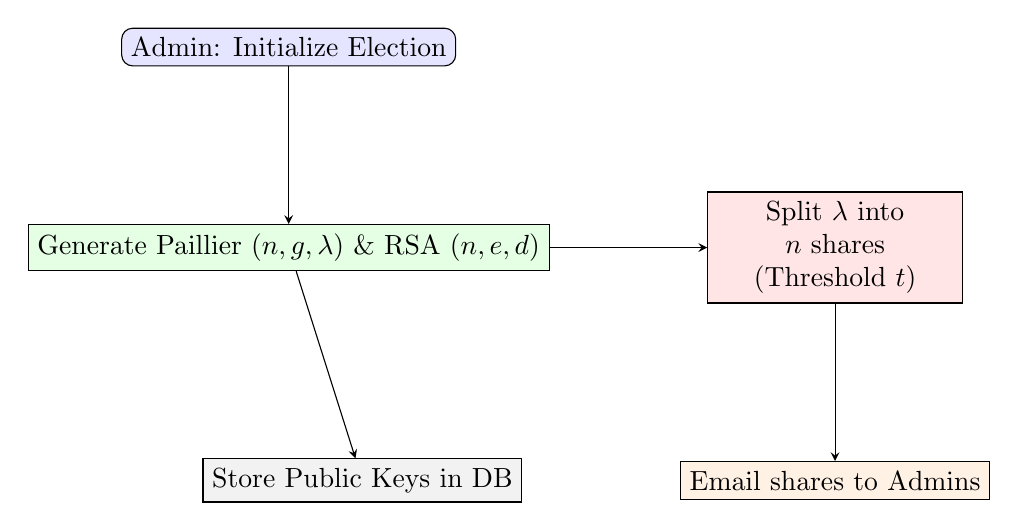
\begin{tikzpicture}[node distance=2cm, auto, >=stealth]
            \node[draw, rounded corners, fill=blue!10] (gen) {Admin: Initialize Election};
            \node[draw, below=of gen, fill=green!10] (keys) {Generate Paillier $(n, g, \lambda)$ \& RSA $(n, e, d)$};
            \node[draw, right=of keys, fill=red!10, text width=3cm, align=center] (shamir) {Split $\lambda$ into $n$ shares (Threshold $t$)};
            \node[draw, below=of shamir, fill=orange!10] (email) {Email shares to Admins};
            \node[draw, left=of email, fill=gray!10] (db) {Store Public Keys in DB};
            
            \draw[->] (gen) -- (keys);
            \draw[->] (keys) -- (shamir);
            \draw[->] (shamir) -- (email);
            \draw[->] (keys) -- (db);
        \end{tikzpicture}
    }
\end{frame}

\begin{frame}{Distributed Trust: Shamir's Secret Sharing}
    \begin{itemize}
        \item The master decryption key $\lambda$ is never stored in one piece.
        \item It is represented as a polynomial $f(x)$ where $f(0) = \lambda$.
        \item Each administrator receives a point $(x_i, f(x_i))$.
        \item To decrypt, $t$ administrators must provide their points to reconstruct $f(x)$ via Lagrange interpolation.
    \end{itemize}
    \vspace{0.5cm}
    \begin{equation*}
        L(x) = \sum_{j=1}^{t} y_j \prod_{k=1, k \neq j}^{t} \frac{x - x_k}{x_j - x_k}
    \end{equation*}
\end{frame}

\begin{frame}{Voter Authentication: RSA Blind Signatures}
    \textbf{Mathematical formulation for anonymity:}
    \begin{enumerate}
        \item \textbf{Blinding (Client):} Voter generates token $T$ and random $r$.
        \begin{equation*} T' = T \cdot r^e \pmod n \end{equation*}
        \item \textbf{Signing (Server):} Server verifies eligibility and signs blinded $T'$.
        \begin{equation*} S' = (T')^d \pmod n \end{equation*}
        \item \textbf{Unblinding (Client):} Voter removes the factor $r$.
        \begin{equation*} S = S' \cdot r^{-1} = (T \cdot r^e)^d \cdot r^{-1} = T^d \pmod n \end{equation*}
    \end{enumerate}
    \centering \textit{The server signs the token without knowing its value, decoupling identity from the vote.}
\end{frame}

\begin{frame}[fragile]{The Voting Flow}
    \resizebox{\textwidth}{!}{
        \begin{tikzpicture}[node distance=2.5cm, auto, >=stealth]
            \node[draw, circle, fill=cyan!10] (voter) {Voter};
            \node[draw, rectangle, right=of voter, fill=orange!10, text width=3cm, align=center] (sig) {
                \textbf{Credential Acquisition}\\
                Obtain Blind Signature $(T, S)$
            };
            \node[draw, rectangle, right=of sig, fill=violet!10, text width=3.5cm, align=center] (encrypt) {
                \textbf{Ballot Encryption}\\
                Encode choice $\vec{v}$\\
                Encrypt with Paillier\\
                Generate ZKPs
            };
            \node[draw, rectangle, right=of encrypt, fill=fuchsia!10, text width=3cm, align=center] (server) {
                \textbf{Voting Server}\\
                Verify $(T, S)$\\
                Verify ZKPs\\
                Homomorphic Agg.
            };
            
            \draw[->] (voter) -- (sig);
            \draw[->] (sig) -- (encrypt);
            \draw[->] (encrypt) -- node[above] {Payload} (server);
        \end{tikzpicture}
    }
\end{frame}

\begin{frame}{Zero-Knowledge Proofs: Individual Validity}
    \textbf{Disjunctive OR-Proof (Individual Choice)}
    To prove $v_i \in \{0, 1\}$ without revealing the actual vote, we use a \textbf{CDS (Cramer-Damgård-Schoenmakers)} proof:
    \begin{itemize}
        \item The voter provides two transcript proofs: one for $v_i=0$ and one for $v_i=1$.
        \item One proof is real (using the witness $r_i$), while the other is simulated.
        \item The verifier checks that the sum of challenges equals the public challenge: $c = c_0 + c_1 \pmod n$.
    \end{itemize}
    \centering \textit{This ensures that each encrypted value is a valid binary vote.}
\end{frame}

\begin{frame}{Zero-Knowledge Proofs: Ballot Consistency}
    \textbf{Sum Proof (Exactly-One Constraint)}
    To prove $\sum_{i=1}^k v_i = 1$ efficiently across all $k$ candidates:
    \begin{itemize}
        \item Let $C_i = g^{v_i} r_i^n \pmod{n^2}$. The voter chooses $r_1, \dots, r_{k-1}$ randomly.
        \item The last randomness is forced: 
        \begin{equation*} r_k = \left( \prod_{i=1}^{k-1} r_i \right)^{-1} \pmod n \end{equation*}
        \item \textbf{Verification:} The server checks if $\prod_{i=1}^k C_i \equiv g^1 \pmod{n^2}$.
    \end{itemize}
    \centering \textit{This mathematical constraint forces the sum to be 1 without leaking which candidate was selected.}
\end{frame}

\begin{frame}[fragile]{The Tallying Process}
    \textbf{Additive Homomorphic Property:}
    The Paillier cryptosystem allows for the addition of plaintexts by multiplying their ciphertexts.
    \begin{equation*}
        E(m_1) \times E(m_2) \pmod{n^2} = E(m_1 + m_2 \pmod n)
    \end{equation*}
    \vspace{0.5cm}
    \resizebox{\textwidth}{!}{
        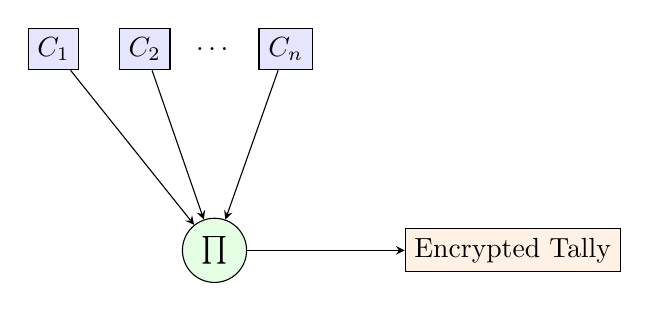
\begin{tikzpicture}[node distance=2cm, auto, >=stealth]
            \node[draw, rectangle, fill=blue!10] (b1) {$C_1$};
            \node[draw, rectangle, right=0.5cm of b1, fill=blue!10] (b2) {$C_2$};
            \node[right=0.2cm of b2] (dots) {$\dots$};
            \node[draw, rectangle, right=0.2cm of dots, fill=blue!10] (bn) {$C_n$};
            \node[draw, circle, below=of dots, fill=green!10] (sum) {$\prod$};
            \node[draw, rectangle, right=of sum, fill=orange!10] (res) {Encrypted Tally};
            
            \draw[->] (b1) -- (sum);
            \draw[->] (b2) -- (sum);
            \draw[->] (bn) -- (sum);
            \draw[->] (sum) -- (res);
        \end{tikzpicture}
    }
\end{frame}

\begin{frame}{Threshold Decryption \& Results}
    \begin{itemize}
        \item \textbf{Phase 1:} Election is CLOSED. No more ballots accepted.
        \item \textbf{Phase 2:} Admins submit their Shamir key shares.
        \item \textbf{Phase 3:} Once threshold $t$ is reached, the server reconstructs $\lambda$.
        \item \textbf{Phase 4:} Master aggregate ciphertext is decrypted.
        \item \textbf{Phase 5:} Results are published and verified against candidate counts.
    \end{itemize}
    \centering \textit{Integrity is maintained because only a valid threshold of admins can reveal the count.}
\end{frame}

\begin{frame}{Security Guarantees \& Conclusion}
    \begin{itemize}
        \item \textbf{End-to-End Verifiability:} Voters can verify their vote was counted using their receipt token.
        \item \textbf{Receipt-Freeness:} Voters cannot prove how they voted to third parties, preventing coercion.
        \item \textbf{Robustness:} Up to $n-t$ admins can be offline or malicious without stopping the election.
        \item \textbf{Privacy:} Absolute anonymity through blind signatures and homomorphic encryption.
    \end{itemize}
    \vspace{1cm}
    \centering \Large \textbf{SigmaVote: Secure. Anonymous. Verifiable.}
\end{frame}

\begin{frame}
    \vspace{2cm}
    \centering
    \Huge Thank You!
    
    \vspace{1cm}
    \large Any Questions?
\end{frame}

\end{document}
